\chapter{数据获取与预处理}
本章将从系统使用的数据集,情感词典和预处理流程三方面进行介绍。
\section{数据集}
为了评估数据模型的准确性以及训练模型以便展示等目的,本文针对语句级和情感级两个任务获取了以下数据集。
\subsection{语句级数据集}
\begin{center}
\begin{longtabu} to 0.8\textwidth{X|X[3]}
\hline
名称 & 手机评论数据集\\
\hline
数据总数 & 2700条\\
语言 & 中文\\
比例 & 正向:负向=1700:1000\\
词数最大值 & 300词数量级\\
90\%词数 & 50词数量级\\
情感分类准确度 & 较为正确\\
语句特点 & 语句较为规范,感情较为强烈\\
获取方式 & 实验室内部资源\\
主要用途 & 初期评估模型可行性及模型展示\\
词频统计 & 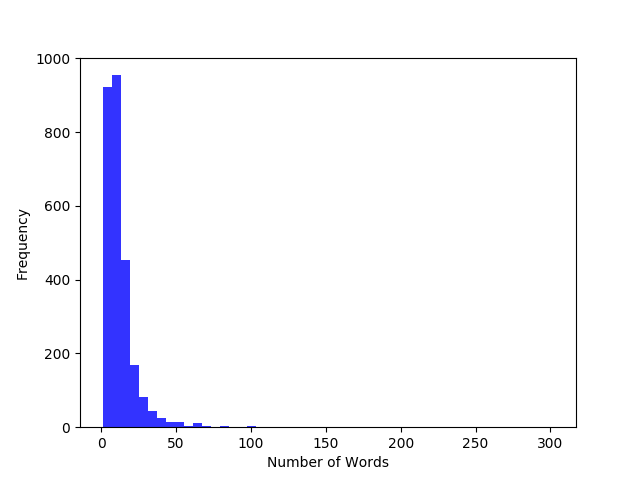
\includegraphics[width=0.6\textwidth, height=0.3\textwidth]{graphic/wordsnum_mobile.png}\\
\hline
%\caption{Mobile Dataset Word Number}
名称 & NLPCC 2014 SCDL数据集\\
\hline
数据总数 & 中文12500条,英文12485条,共24985条\\
官方测试集数据总数 & 中文2500条,英文2500条\\
语言 & 中文,英文\\
比例 & 中文 正向:负向=1700:1000\\
测试集比例 & 中文 正向:负向=1250:1250 英文 正向:负向=1250:1250\\
词数最大值 & 1000词数量级\\
90\%词数 & 200词数量级\\
情感分类准确度 & 不够准确\\
语句特点 & 语句较为口语化,有广告等中性语句\\
获取方式 & \url{http://tcci.ccf.org.cn/conference/2014/pages/page04_sam.html}(Accessed at: 5/21/2017)\\
主要用途 & 评估模型性能\\
词频统计 & 
中文\newline
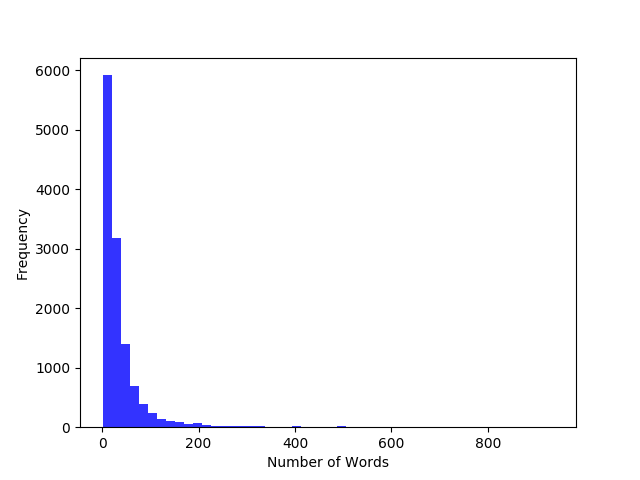
\includegraphics[width=0.6\textwidth, height=0.3\textwidth]{graphic/wordsnum_nlpcc_zh.png}
英文
\newline
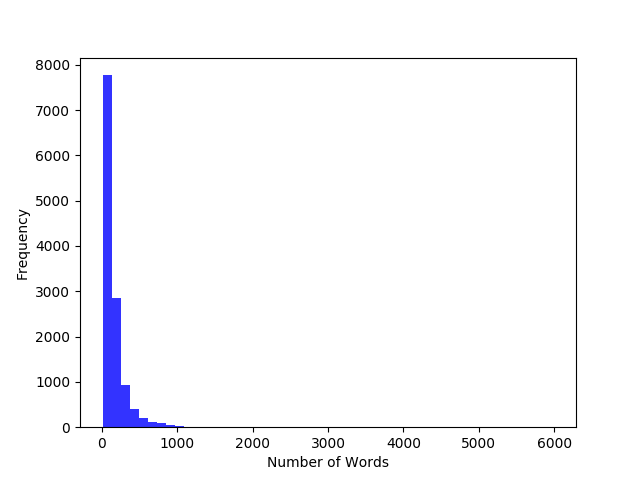
\includegraphics[width=0.6\textwidth, height=0.3\textwidth]{graphic/wordsnum_nlpcc_en.png}\\
\hline
名称 & 携程数据集\\
\hline
数据总数 & 250463条\\
语言 & 中文\\
比例 & 正向:负向=193138:57325\\
词数最大值 & 1750词数量级\\
90\%词数 & 250词数量级\\
情感分类准确度 & 不够准确\\
语句特点 & 语句较为口语化\\
获取方式 & 通过selenium模拟浏览器爬取到388067条带评分的携程酒店评论,其中评分小于4.0的定为负向,评分等于5的定为正向\\
主要用途 & 模型展示及标注实体数据集\\
词频统计 & 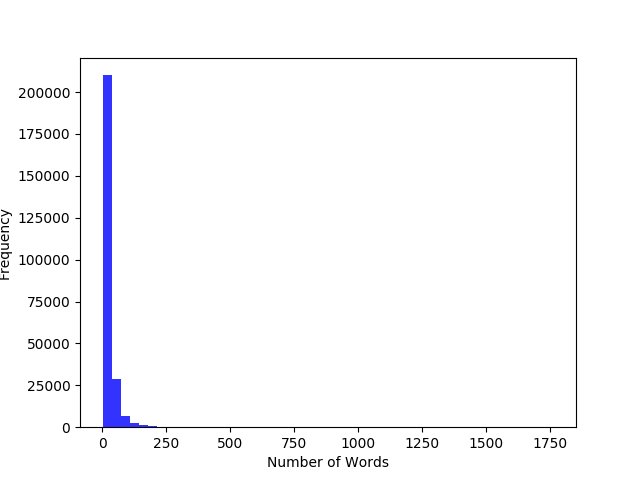
\includegraphics[width=0.6\textwidth, height=0.3\textwidth]{graphic/wordsnum_xiecheng.png}\\
\hline
\end{longtabu}
\end{center}  
\subsection{实体级数据集}
\begin{center}  
\begin{longtabu} to 0.8\textwidth{X|X[3]} 

\hline
名称 & SemEval2014Task4数据集\\
\hline
数据总数 & Laptop子数据集为3045条,Restaurants子数据集为3041条\\
语言 & 英文\\
词数最大值 & 80词数量级\\
90\%词数 & 50词数量级\\
情感分类准确度 & 较为正确\\
语句特点 & 语句较为规范,感情较为强烈\\
获取方式 & \url{http://alt.qcri.org/semeval2014/task4/}(Accessed at: 5/21/2017),取其中已标注的训练数据部分\\
主要用途 & 评估模型可行性及模型展示\\
词频统计 & 
Laptop\newline
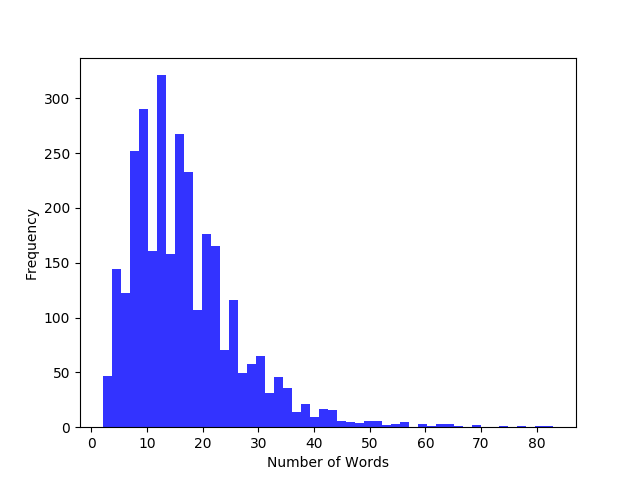
\includegraphics[width=0.6\textwidth, height=0.3\textwidth]{graphic/wordsnum_semval14_laptop.png}
\newline
Restaurant
\newline
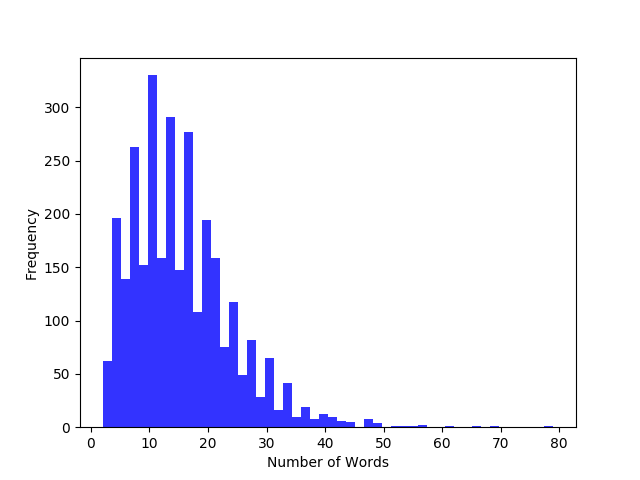
\includegraphics[width=0.6\textwidth, height=0.3\textwidth]{graphic/wordsnum_semval14_restaurants.png}\\
\\
\hline
名称 & 携程实体数据集\\
\hline
数据总数 & 6947条\\
语言 & 中文\\
词数最大值 & 100词数量级\\
90\%词数 & 20词数量级\\
情感分类准确度 & 较为正确\\
语句特点 & 语句较为规范,感情较为强烈\\
获取方式 & 对携程数据集进行过滤,取长度为10-100词之间,名词类词语只能为特定实体的语句进行手工标注实体和实体极性得到\\
主要用途 & 评估模型可行性及模型展示\\
词频统计 & 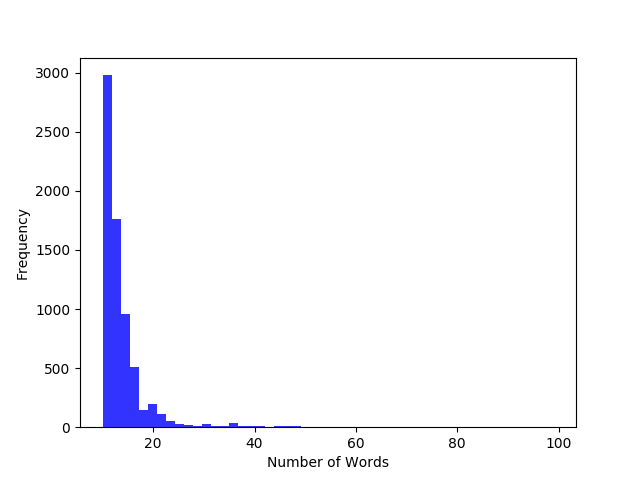
\includegraphics[width=0.6\textwidth, height=0.3\textwidth]{graphic/wordsnum_xiechengABSA.png}\\
\hline
\end{longtabu}  
\end{center}  

携程实体数据集所用到的实体如下:
\begin{itemize}
\item 地铁,整体,态度,服务员,性价比
\item 价格,前台,早餐,交通,位置
\item 设施,环境,房间,酒店
\end{itemize}
该实体集合是通过统计携程数据集上出现频率为前20的名词,经过过滤后得到的。

\section{情感词典}
由于知识模型可以同时支持中/英文分析,故情感词典主要由以下两种语言共六个词典组成。
\subsection{中文情感词典}
\begin{enumerate}
\item Hownet(知网)情感词典\cite{hownet}:语言为中英双语,但本文主要使用中文部分。该词典为董振东和董强建立的情感分析用语集,包括主张词语,正面/负面情感词语,正面/负面评价词语,程度级别词语,并为程度级别词语划分强度等级,但其中有一些不符合构词法的词语,如“噲”,“媢”,“媢嫉”,“忺”,“安”,“巴”等在正面情感词典中出现的词。另外词语可能以短语形式出现,如“越...越...”,“abandon oneself to despaire”等。
\item NTUSD台湾大学情感词典:台湾大学自然语言处理实验室提供的情感词典,包括正面词汇2810个和负面词汇8276个,极性划分较为准确,且包含各种词性,如“一下子爆发”,“一下子爆发的一连串,“一巴掌”。
\item DUTIR情感词汇本体库:大连理工大学信息检索研究室整理和标注的中文情感词库,具有词性,情感分类,强度,极性和辅助情感分类,强度,极性等特征,划分详细。包含各种词性,但以成语和俗语为主体。
\end{enumerate}
\subsection{英文情感词典}
\begin{enumerate}
\item SentiWordNet\cite{sentiwordnet} \cite{sentiwordnet3}:基于WordNet3.0,具有语义,正向评分PosScore和负向评分NegScore等信息,本文中取PosScore-NegScore之差作为其分数。
\item Opinion Lexicon:Bing Liu等\cite{huliu2004a} \cite{huliu05a} 整理的极性情感词典,仅包含单词本身,不包含短语,但包括单词的各种变形形式。
\item 匹兹堡大学MPQA主观性词典\cite{mpqa}:是MPQA(Multi-Perspective Question Answering,多方面问答)系统所用到的词典,具有情绪词,词性,情感强弱等。
\end{enumerate}